
\procTitle{Архитектура жилой застройки в развитии г.~Магадана}

\procAuthor{Судчак~Н.\,А., Лунегова~А.\,А., Болотин~А.\,В.}
\procEmail{sudchak99@mail.ru, laaru@rambler.ru, alexandr\_bolotin@mail.ru}
\procOrganization{СВГУ}
\procCity{Магадан}


\makeProcTitle
\index{l@Лунегова~А.\,А.}
\index{b@Болотин~А.\,В.}
\index{s@Судчак~Н.\,А.}

История развития человеческого общества на всех этапах своего развития отражалась в памятниках архитектуры. Архитектурные сооружения являются наиболее доступными для обозрения памятниками эпохи. Функциональная сторона архитектуры, ее польза, надобность является неотъемлемым элементом всякого сооружения. Любое здание строится для того, чтобы удовлетворить известному назначению, определенным функциям. От~функционального назначения, будь то жилое, общественное или промышленное здание, зависят тип архитектурного сооружения, количество и~состав помещений в нем, их расположение, группировка и размеры.

Типы зданий складывались не сразу, они определялись исторической ситуацией в стране, политическим устройством, религиозными и идеологическими требованиями, бытом, народными традициями, климатическими и прочими факторами. В ходе исторического развития видоизменялись и традиционные типы зданий, например, жилые дома, административные сооружения, театры, больницы и другие. Современные жилые дома отличаются от жилых домов XVII--XIX~вв., от домов средневековья, а ратуши эпохи Возрождения – от современных административных зданий [3].

Объектом исследования выбрана архитектура жилой застройки г.~Магадана, а предметом выбран микрорайон <<Автотек>> г. Магадана. Микрорайон насчитывает 51~дом. По периодам возведения жилые дома получили условные названия: <<сталинка>>, <<хрущевка>>, <<брежневка>>. Их распределение по периодам возведения представлено в таблице.


\begin{wraptable}{l}{7.0cm}
  \caption*{\textbf{Периоды возведения жилых домов\\микрорайона <<Автотэк>> г.~Магадана} }
  \label{tab:sydchak-tab}
  \begin{tabular}{ccc}
\toprule
  Тип дома    & Год постройки & Кол-во \\
\midrule
  <<Сталинки>>    & до 1956       & 3      \\
  <<Хрущёвки>>    & 1956--1964     & 6      \\
  <<Брежневки>>   & 1964--1980     & 13     \\
  Современные & после 1980    & 29     \\\midrule
  Всего       &               & 51\\ \bottomrule
  \end{tabular}


%\end{minipage}
\end{wraptable}


Данные таблицы свидетельствуют о том, что жилой микрорайон <<Автотек>> является носителем истории архитектуры России всех послевоенных пятилеток и постсоветского периода. Рассмотрим кратко архитектуру жилищного строительства каждого периода.

\textbf{<<Сталинки>>}

Большое место в жилищном строительстве принадлежит начавшемуся в 1946~г. крупнопанельному индустриальному домостроению по типовым проектам. Однако большинство жилых домов возводилось по индивидуальным проектам, с излишествами в обработке фасадов. Одной из причин этого было стремление советских зодчих отразить в архитектуре триумфальное завершение Великой Отечественной войны. Концентрация строительства способствовала развитию поточно-скоростных методов производства и широкому внедрению индустриальных изделий и деталей [1].

Здания, сооружавшиеся в СССР с конца 1940-х~гг. до середины 1965-х~гг., преимущественно были в стиле неоклассицизм (сталинский ампир). Различают жилье с улучшенной планировкой и более изысканным фасадом, а для рабочих~--- с упрощенным декором фасада. Для данного типа характерным является кирпичная стеновая конструкция, оштукатуренная по фасаду. Кровля скатная или вальмовая, по деревянным стропилам. Нормативный срок службы зданий 125--150 лет.

Особенностью такого типа является~--- ансамблевый характер застройки. Массовые здания строгого архитектурного стиля с парадным этажом, с~декоративными элементами. Типичным примером <<сталинки>> в стиле неоклассицизма является д.~6 на площади Горького г.~Магадана (рис. 1, 2).

В послевоенной архитектуре украшательства и <<излишества>> достигли особого расцвета.

\begin{figure}[H]
%\begin{changemargin}{-0.5cm}{-1cm}
  \begin{center}
    \begin{minipage}[h]{0.38\linewidth}
        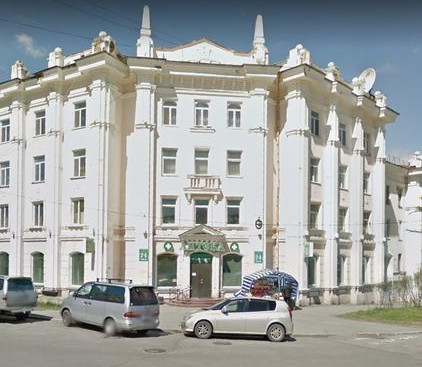
\includegraphics[width=1\textwidth]{authors/sydchak-fig-1.jpg}
        \caption{Дом 6 на Площади Горького}
        \label{fig:sydchak-fig-1}
    \end{minipage}
\hfill
    \begin{minipage}[h]{0.50\linewidth}
        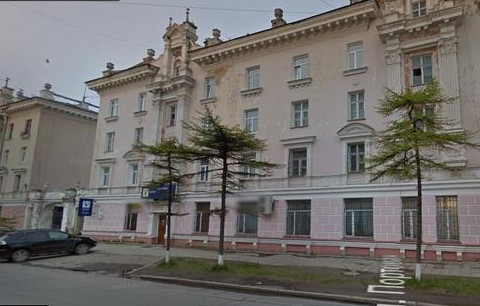
\includegraphics[width=1\textwidth]{authors/sydchak-fig-2.jpg}
        \caption{Дом 3 на улице Портовой}
        \label{fig:sydchak-fig-2}
    \end{minipage}


  \end{center}
%\end{changemargin}

\end{figure}

\vspace{-0.5cm}
\textbf{<<Хрущевки>>}

Вскоре после смерти Сталина, в 1954~г. на Всесоюзном совещании строителей это направление было осуждено, и положено начало строительству зданий, лишённых всякого декора [3].  В ноябре 1955~г. выходит Постановление ЦК КПСС и СМ СССР <<Об устранении излишеств в проектировании и~строительстве>>, положившее конец стилю сталинской архитектуры [4]. На~смену сталинской пришла функциональная типовая архитектура. В~июле 1957~г. ЦК КПСС и Совет Министров СССР приняли постановление <<О развитии жилищного строительства в СССР>>, положившее начало массовому строительству домов, получивших название <<хрущёвки>> по имени Никиты Сергеевича Хрущёва [5].

Для данного типа характерным является панельная или блочная сборная железобетонная стеновая конструкция. Наружные панели и блоки с~уличной стороны окрашены. Предусмотрены балконы.  Кровля может быть скатной и плоской. Нормативный срок службы 125--150~лет. Особенностью такого типа является~--- микрорайонный, строчный характер (рис.~3, 4).

\begin{figure}[H]
\begin{changemargin}{2cm}{2cm}
  \begin{center}
    \begin{minipage}[h]{0.45\linewidth}
        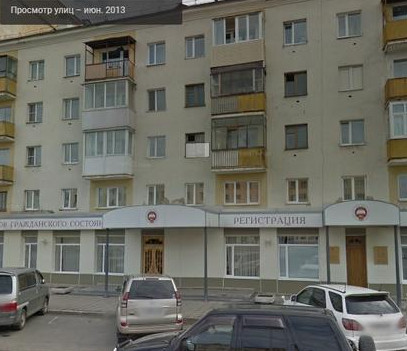
\includegraphics[width=1\textwidth]{authors/sydchak-fig-3.jpg}
        \caption{Фотография дома №\,37 по~пр-ту Карла Маркса}
        \label{fig:sydchak-fig-3}
    \end{minipage}
\hfill
    \begin{minipage}[h]{0.45\linewidth}
        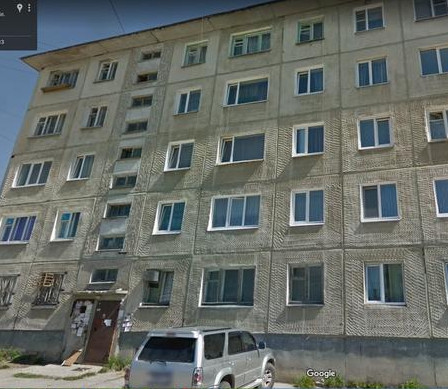
\includegraphics[width=1\textwidth]{authors/sydchak-fig-4.jpg}
        \caption{Фотографяи дома №\,9В по~ул.~Берзина}
        \label{fig:sydchak-fig-4}
    \end{minipage}


  \end{center}
\end{changemargin}

\end{figure}


\textbf{<<Брежневки>>}

Обзор массового жилищного строительства в СССР с 1964 по 1980~гг. показывает, что этот период прежде всего характеризуется непрерывным увеличением его темпов. Событием огромного социального значения явился переход на строительство экономичных квартир, предназначенных для заселения одной семьёй. Этот переход оказался возможным в результате того, что индустриальное домостроение стало генеральной линией жилищного строительства.

Заводское домостроение перешло к производству комплектов жилых домов с различными конструктивными схемами, в результате чего во многих крупных городах индустриальное строительство к 1970~г. достигло 70--85\,\% общего объёма жилищного строительства, а в среднем по стране составляло около 40\,\% [2].

Для данного типа характерным является панельная или блочная сборная железобетонная стеновая конструкция. На этажах располагается много квартир, выходящих в длинный коридор, квартиры малометражные или однокомнатные. Наружные панели и блоки с уличной стороны окрашены. Кровля плоская. Нормативный срок службы 125--150 лет. Особенностью такого типа является~--- микрорайонный, строчный характер (рис. 5).

\begin{figure}[h!]

    \begin{center}
    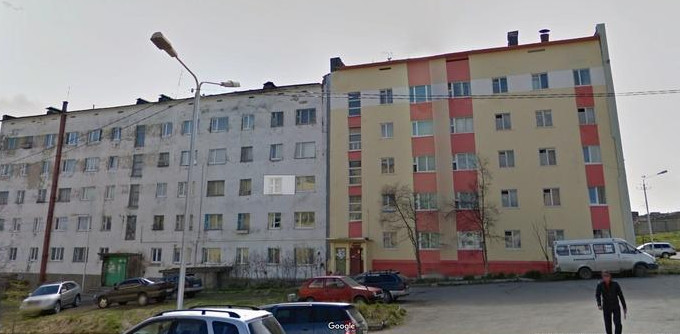
\includegraphics[width=0.7\textwidth]{authors/sydchak-fig-5.jpg}
  \end{center}
  \caption{Дом 15 корпус 1, Марчеканский переулок}
  \label{fig:sydchak-fig-5}

\end{figure}


К концу рассматриваемого периода произошли значительные качественные изменения. Были разработаны и начали внедряться новые улучшенные типы квартир и жилых домов. Квартиры стали просторнее и удобнее, обогатились лоджиями и эркерами. Увеличение количества разнотипных квартир улучшило возможности расселения семей в соответствии с демографией населения. В сериях появились жилые дома с элементами общественного бытового обслуживания. В состав серий были включены также более комфортабельные жилые дома повышенной этажности, оборудованные лифтами и мусоропроводами.

\textbf{<<Современные>>}

После распада СССР многие строительные проекты были заморожены или отменены. Однако теперь не существовало государственного контроля над архитектурным стилем и высотой здания, что давало значительную свободу архитекторам. Финансовые условия позволяли заметно ускорить темпы развития архитектуры.

Современные здания, построенные с 2000-х~гг. по настоящее время, выполнены по индивидуальным проектам. Для данного типа характерным является каркасная железобетонная конструкция из крупноразмерных блоков. Фасады облицованы металлосайдингом, часто имеют утепление. Кровля плоская. Нормативный срок службы 100 лет. Особенностью такого типа является~--- микрорайонный, строчный характер (рис. 6, 7).

\begin{figure}[H]
\begin{changemargin}{-1cm}{-1cm}
  \begin{center}
    \begin{minipage}[h]{0.545\linewidth}
        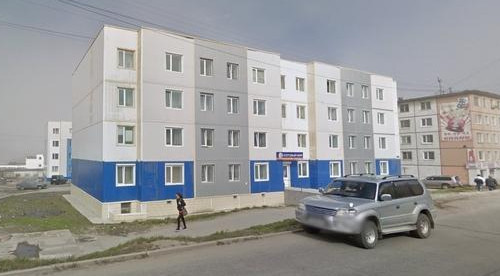
\includegraphics[width=1\textwidth]{authors/sydchak-fig-6.jpg}
        \caption{Дом 15, улица Гагарина }
        \label{fig:sydchak-fig-6}
    \end{minipage}
\hfill
    \begin{minipage}[h]{0.4\linewidth}
        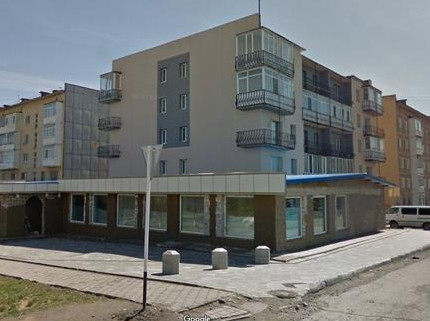
\includegraphics[width=1\textwidth]{authors/sydchak-fig-7.jpg}
        \caption{Дом 23/1, улица Парковая }
        \label{fig:sydchak-fig-7}
    \end{minipage}


  \end{center}
\end{changemargin}

\end{figure}

\vspace{-12pt}
Принятое в исследовании разделение истории советской и постсоветской архитектуры на четыре этапа: до 1956~г., 1956--1964~гг., 1964--1980~гг., с 1980~г. и по настоящее время условно. Эти этапы связаны с определенными моментами качественных изменений в творческой направленности отечественной архитектуры. Все отмеченные нами особенности отечественной архитектуры делают историю ее развития, анализ ее достижений и тенденций особенно ценными для науки и практики, если рассматривать историю предмета не как хронологическую последовательность событий, но как истолкование этих фактов в их диалектическом развитии, в борьбе нового со старым, отживающим. Без такой истории нельзя сколько-нибудь обоснованно наметить перспективы дальнейшего развития архитектуры, ибо определение этих перспектив требует научной теории, т.\,е. истории архитектуры в ее наиболее общем виде.

Анализ характера изменений архитектуры жилой застройки города показал тесную связь эволюции стилей отечественной архитектуры в зависимости от развития Магадана и Российской Федерации в целом.

\begin{thebibliography}{99}
\bibitem{}Архитектура послевоенных пятилеток 1945--1968~гг. // Строй-Сервер.~--- 2007.~--- URL: http://stroy-server.ru/notes/arkhitektura-poslevoennykh-pyatiletok-1945-1968-gg/ (дата обращения 10.03.2020).
\bibitem{}Архитектура России // Новости архитектуры.~--- Дата обновления: 02.03.2017.~--- URL: http://global.proekt-a.com/articles/161-site-texts/seo-newsrus/5341-arkhitektura-rossii/ (дата обращения 10.03.2020).
\bibitem{}Постановление № 1871 ЦК КПСС и СМ СССР от 4 ноября 1955 г. <<Об устранении излишеств в проектировании и строительстве>> // Википедия~--- свободная энциклопедия.~--- Дата обновления: 24.04.2020.~--- URL:https://ru.wikipedia.org/wiki/Об\_устранении\_излишеств\_в\_про\-ек\-ти\-ро\-ван\-ии\_и\_строительстве (дата обращения 10.03.2020).
\bibitem{}Постановление ЦК КПСС и СМ СССР от 31 июля 1957 г. № 931 <<О развитии жилищного строительства в СССР>>.~--- 2011.~--- URL: http://www.libussr.ru/doc\_ussr/ussr\_5213.htm (дата обращения 10.03.2020).

\end{thebibliography}
